\documentclass{standalone}
%
\usepackage{tikz}
\usetikzlibrary{backgrounds}
\usetikzlibrary{plotmarks}
\usetikzlibrary{arrows}
\usetikzlibrary{arrows.meta}
\tikzset{>={Latex[width=5mm,length=10mm]}}
\usetikzlibrary{decorations, decorations.text}
%
\usepackage{amsmath}
\usepackage{xcolor}
%
\definecolor{space}{HTML}{0A2543}
\definecolor{earth}{HTML}{0089FA}
\definecolor{mars}{HTML}{DC7B4E}
\definecolor{dida}{HTML}{FFDE00}
\definecolor{title}{HTML}{FBA706}
\definecolor{moon}{HTML}{AFAFAF}
\definecolor{lsb}{HTML}{D8603E}
%
\usepackage{mathptmx}
\usepackage{fontspec}
\setmainfont{Montserrat}
%
\title{Metodo di Eratostene}
\begin{document}
	\tikzset{partial ellipse/.style args = {#1:#2:#3}{insert path={+ (#1:#3) arc (#1:#2:#3)}}}
	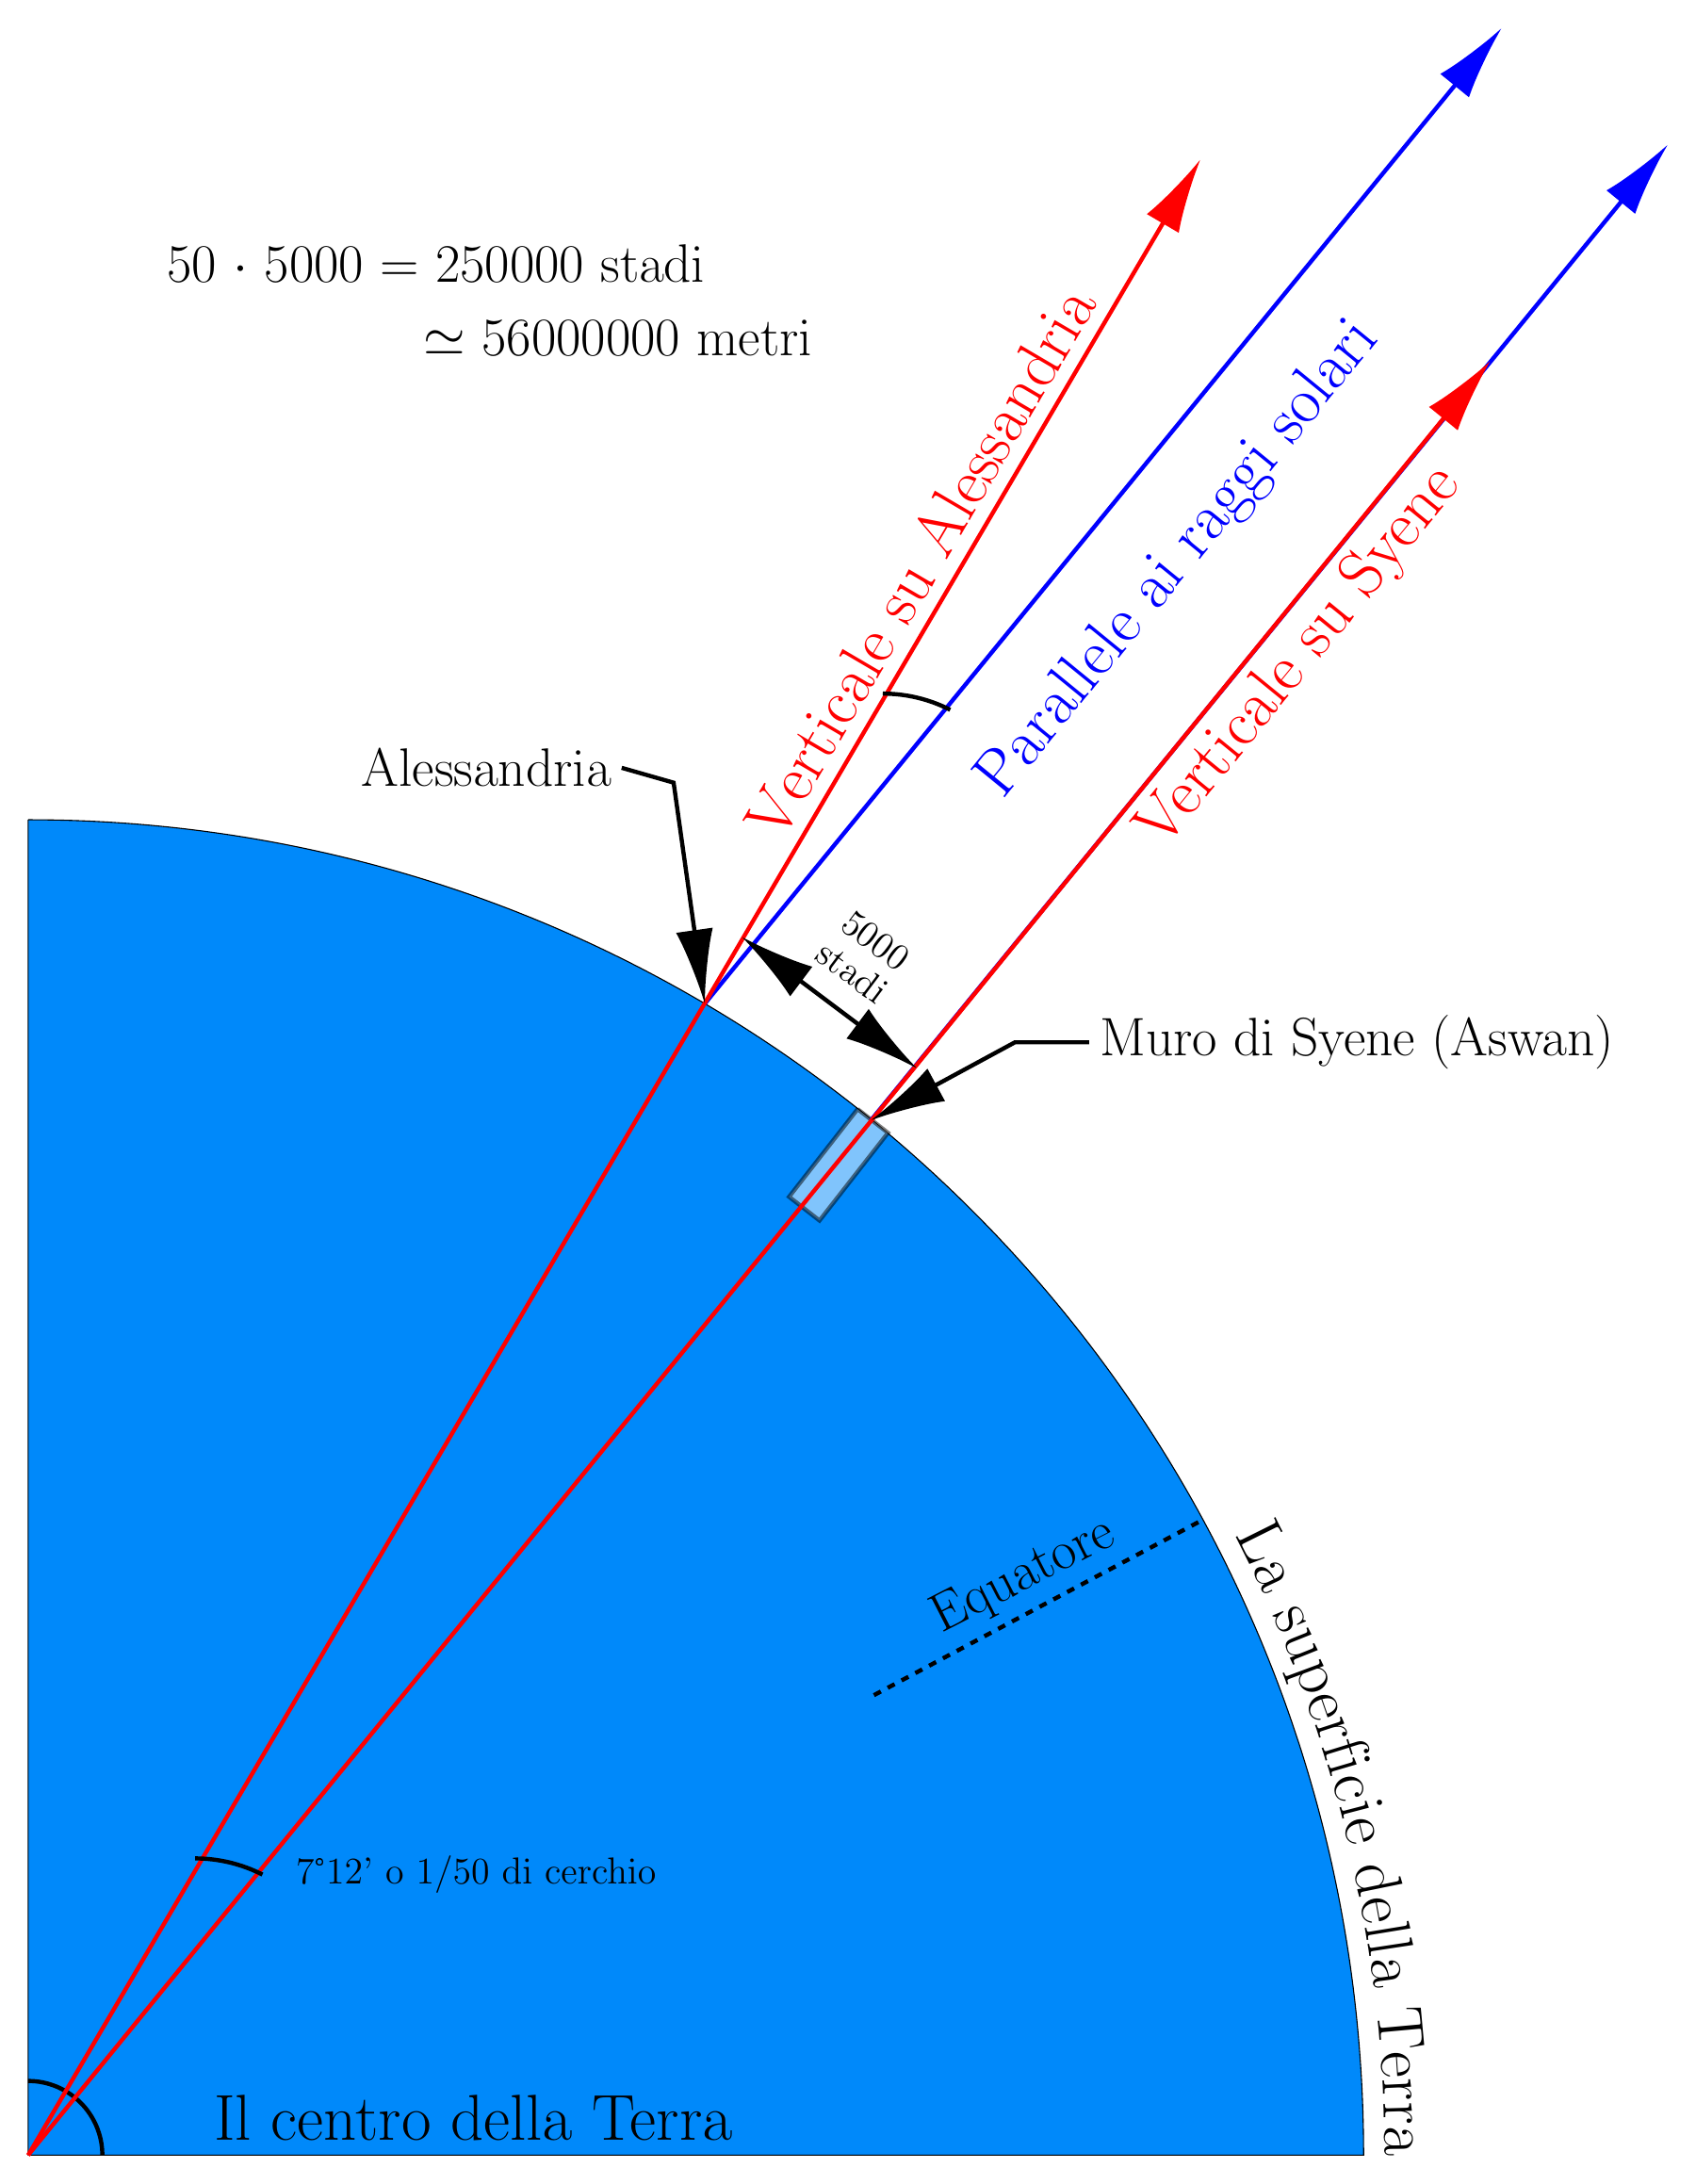
\begin{tikzpicture}%[y=.2cm, x=.7cm,font=\sffamily]%[background rectangle/.style={fill=space},show background rectangle]
		\begin{scope}
			%superficie della terra
			\draw [fill=earth] (-11,1) arc(90:0:18) -- (-11,-17) -- (-11,1);
			%etichetta sulla superficie
			\draw [decorate,decoration={text along path, raise=8pt, text align=right, text={|\fontsize{27}{28}\selectfont|La superficie della Terra}}] (-11,1) arc(90:0:18);
			%centro della terra con etichetta
			\draw [ultra thick] (-11,-16) arc(90:0:1);
			\node at (-5,-16.5) () {\fontsize{27}{28}\selectfont Il centro della Terra};
			%pozzo
			\draw[rotate around={-38:(0.18,-2.9)},ultra thick,fill=white, opacity=0.5] (0.18,-2.9) -- (0.7,-2.9) -- (0.7,-4.4) -- (0.18,-4.4) -- (0.18,-2.9);
			%frecce
			\begin{scope}%[>=latex]
				%etichetta verticale Alessandria
				\draw [decorate,decoration={text along path, raise=6pt, text align=center, text={|\fontsize{24}{25}\selectfont\color{red}|Verticale su Alessandria}}] (-1.88,-1.48) -- (4.8,9.9);
				%etichetta parallele
				\draw[shift={(-1,0.8)}] [decorate, decoration={text along path, raise=2pt, text align=center, text={|\fontsize{24}{25}\selectfont\color{blue}|Parallele ai raggi solari}}] (0.36,-3.05) -- (11.1,10.1);
				%raggi sole Syene ed etichetta verticale Syene
				\draw[arrows=->, color=blue, ultra thick] (0.36,-3.05) -- (11.1,10.1) node [below, midway, sloped] (TextNode) {\textcolor{red}{\fontsize{24}{25}\selectfont Verticale su Syene}};
				%raggi sole Alessandria
				\draw[arrows=->, color=blue, ultra thick, shift={(-2.24,1.57)}] (0.36,-3.05) -- (11.1,10.1);
				%verticali Alessandria e Syene
				\draw[arrows=->, color=red, ultra thick] (-11,-17) -- (4.8,9.9);
				\draw[arrows=->, color=red, ultra thick, rotate around={-8.75:(-11,-17)}] (-11,-17) -- (4.8,9.9);
				%5000 stadi
				\draw[arrows=<->,color=black, ultra thick] (-1.38,-0.58) -- (0.98,-2.35);
				\draw [decorate,decoration={text along path, raise=10pt, text align=center, text={|\fontsize{15}{16}\selectfont\color{black}|stadi}}] (-1.38,-0.58) -- (0.98,-2.35);
				\draw [decorate,decoration={text along path, raise=25pt, text align=center, text={|\fontsize{15}{16}\selectfont\color{black}|5000}}] (-1.38,-0.58) -- (0.98,-2.35);
				%freccia Alessandria
				\draw[arrows=<-, ultra thick] (-1.88,-1.48) -- (-2.3,1.5) -- (-3,1.7) node [left] (TextNode) {\textcolor{black}{\fontsize{21}{22}\selectfont Alessandria}};
				%freccia Syene
				\draw[arrows=<-, ultra thick] (0.36,-3.05) -- (2.3,-2) -- (3.3,-2) node [right] (TextNode) {\textcolor{black}{\fontsize{21}{22}\selectfont Muro di Syene (Aswan)}};
			\end{scope}
			%equatore
			\draw[-,dashed, ultra thick, rotate around={1:(0.4,-10.8)}] (0.4,-10.8) -- (4.9,-8.5) node [above, midway, sloped] (TextNode) {\textcolor{black}{\fontsize{21}{22}\selectfont Equatore}};
			%1/50 di cerchio
			\draw [ultra thick] (-8.75,-13) arc(90:63:2) node [right] (TextNode) {\textcolor{black}{\fontsize{15}{16}\selectfont $\;$ 7\textdegree 12' o 1/50 di cerchio}};
			\draw [ultra thick] (0.52,2.7) arc(90:63:2);
			%
			\node at (-5.5,8.5) () {\textcolor{black}{\fontsize{21}{22}\selectfont 50 $\cdot$ 5000 $=$ 250000 stadi}};
			\node at (-3.05,7.5) () {\textcolor{black}{\fontsize{21}{22}\selectfont $\simeq$ 56000000 metri}};
		\end{scope}
		%
	\end{tikzpicture}
%
\end{document}
